\FloatBarrier
\begin{figure}[!h]
\centering
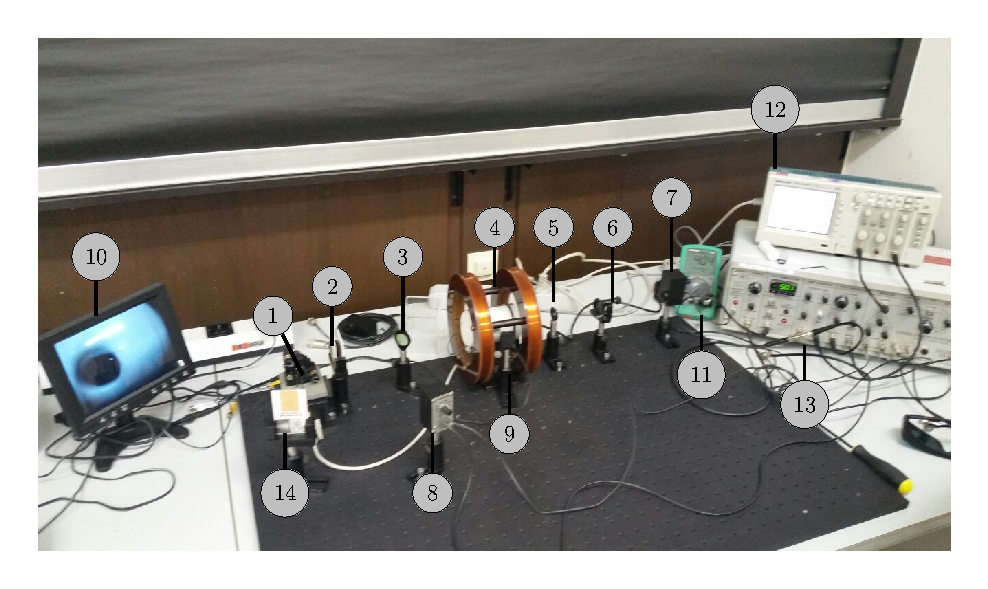
\includegraphics[scale=1]{../Grafiken/Diodenlaser_Aufbau_Nr.pdf}
\caption{Vollständiger Aufbau nach Durchführung des Versuchs, mit dem das Absorptionsspektrum von 
	Rubidium aufgenommen wurde. Die Nummerierten Bauteile sind im Einzelnen:
	(1) Diodenlaser \& Gitter, (2) ND-Filter, (3) Strahlteiler 50:50, (4) Rubidiumkammer \& Helmholtzspulen,
	(5) Blende, (6) ND-Filter, (7) Photodiode, (8) Photodiode, (9) Kamera, (10) Kamera-Monitor,
	(11) Voltmeter, (12) Digitales Oszilloskop, (13) Steuerungseinheit, (14) IR-Sichtkarte.
	\label{fig:diodenlaser_aufbau_nr}}
\end{figure}
\FloatBarrier